\documentclass[a4paper]{ctexart}
\usepackage{ctex}
\usepackage{times}
\usepackage{setspace}
\usepackage{fancyhdr}
\usepackage{graphicx}
\usepackage{wrapfig}
\usepackage{array}
\usepackage{fontspec,xunicode,xltxtra}
\usepackage{titlesec}
\usepackage{titletoc}
\usepackage[titletoc]{appendix}
\usepackage[top=29mm,bottom=29mm,left=31.8mm,right=31.8mm]{geometry}
\usepackage{enumerate}
\usepackage{caption}
\usepackage{abstract}
\usepackage{amsmath}
\usepackage{booktabs}
\usepackage{multirow}
\usepackage{cite}
\setmainfont{Times New Roman}
\setCJKmainfont[BoldFont={Songti SC Bold}]{SimSun}
\setCJKfamilyfont{heiti}{SimHei}
\renewcommand{\heiti}{\CJKfamily{heiti}\fontspec{Times New Roman}}

\newcommand{\mycaptionfont}{\heiti\zihao{5}}
\captionsetup[figure]{name={\mycaptionfont 图},labelsep=period}
\renewcommand{\captionfont}{\mycaptionfont}
\renewcommand{\captionlabelfont}{\mycaptionfont}

%---------------------------------------------------------------------
%	页眉页脚设置
%---------------------------------------------------------------------
\fancypagestyle{plain}{\pagestyle{fancy}}%改变章节首页页眉
\pagestyle{fancy}
\lhead{\kaishu~无线射频识别技术课程作业~}
\rhead{\kaishu~纪港~尹达恒~郭星宇~孙硕~孙瑜博~王雷}
\cfoot{\thepage}

%---------------------------------------------------------------------
%	目录页设置
%---------------------------------------------------------------------
\setcounter{tocdepth}{3}
\titlecontents{section}[2em]{\vspace{0.1\baselineskip}\songti\zihao{-4}}{\thecontentslabel\ }{}
{\hspace{.5em}\titlerule*[4pt]{$\cdot$}\contentspage}
\titlecontents{subsection}[4em]{\vspace{0.1\baselineskip}\songti\zihao{-4}}{\thecontentslabel\ }{}
{\hspace{.5em}\titlerule*[4pt]{$\cdot$}\contentspage}
\titlecontents{subsubsection}[6em]{\vspace{0.1\baselineskip}\songti\zihao{-4}}{\thecontentslabel\ }{}
{\hspace{.5em}\titlerule*[4pt]{$\cdot$}\contentspage}

\ctexset {
	section = {
		number = \arabic{section},
		format = \zihao{4}\bfseries,
	},
	subsection = {
		number = \arabic{section}.\arabic{subsection},
		format = \zihao{-4}\bfseries,
	},
	subsubsection = {
		number = \arabic{section}.\arabic{subsection}.\arabic{subsubsection},
		format = \zihao{-4}\bfseries,
	}
}

\begin{document}
%---------------------------------------------------------------------
%	封面设置
%---------------------------------------------------------------------
\begin{titlepage}
\newgeometry{top=30mm,bottom=30mm,left=20mm,right=20mm}
	\begin{center}
    
\includegraphics[width=0.9\textwidth]{figure//Njust.png}\\
    \vspace{10mm}
    \zihao{2}\kaishu{物联网工程学院}\\[0.5cm]
    \zihao{2}\kaishu{无线射频识别技术课程作业}\\[2.5cm]
    \zihao{2}\kaishu{高频RFID标签和读写器芯片的结构与功能分析}\\
    \zihao{3}\kaishu{——以复旦微电子FM13HS02芯片和FM17550芯片为例}\\[2.5cm]
	\vspace{\fill}
	\setlength{\extrarowheight}{3mm}
	{\songti\zihao{3}	
		\begin{tabular}{rl}
			{\makebox[4\ccwd][s]{班\qquad 级:}}& ~\kaishu 物联1601\\
			{\makebox[4\ccwd][s]{组\qquad 长:}}& ~\kaishu 纪港 \\
			{\makebox[4\ccwd][s]{组\qquad 员:}}& ~\kaishu 尹达恒、郭星宇、孙硕、孙瑜博、王雷 \\
			{\makebox[4\ccwd][s]{指导老师:}} & ~\kaishu 孙子文\\
		\end{tabular}
	}\\[2cm]
	\vspace{\fill}
	\zihao{4}
	2018\textasciitilde 2019第二学期\\
	\today
	\end{center}
\restoregeometry
\end{titlepage}


\tableofcontents
\newpage


\begin{spacing}{1.5}
\songti\zihao{-4}
\section{高频RFID射频识别系统硬件结构简介}
一个完整的RFID系统通常由标签 (Tag or Transponder) 、阅读器 (Interrogator or Reader) 和数据管理系统组成。标签一般包含天线、调制/解调器、编码/解码器以及储存器或微控制器等单元;阅读器由天线、射频收发模块和控制单元组成, 其中控制模块通常包含放大器、解码和纠错电路、微处理器、时钟电路、标准接口以及电源电路等\cite{RN97}。
\subsection{电子标签的硬件结构简介}
电子标签的硬件结构按照功能可以划分为三个主要部分:天线、模拟前端(射频前端)和控制电路(如图\ref{f0})。电子标签中的射频信号调制器和解调器包含于模拟前端中,编码/解码器、储存器或微控制器等单元包含于控制电路中。电子标签工作时,其天线接收由读写器发出的信号,该信号通过射频前端电路中的解调器和解码器等部件的处理,进入电子标签的控制电路,由控制电路对数据流做各种逻辑处理,再经过射频前端的编码和调制发送到读写器。依照控制电路的结构,电子标签可分为不可编程电子标签和可编程电子标签。

不可编程电子标签的控制电路硬件结构包括地址和安全逻辑形成电路、IO寄存器和存储器等部分。其中地址和安全逻辑电路是控制电路的主要部分,它控制整个芯片的处理进程,并且和专用IO寄存器互相配合完成数据交换、授权、加密及密匙管理等功能。存储器主要包括ROM、EEPROM或FRAM,ROM主要存放永久数据,EEPROM或FRAM连接芯片内部逻辑电路的地址线和数据线进行数据交换。电子标签的工作受存储器中的程序控制,控制程序一旦确定就被固定在芯片存储器中,不能改变\cite{RN98}。

可编程电子标签的控制电路硬件结构除存储器外还包括一个微控制器。微控制器可以运行微操作系统程序,控制电子标签的数据转换、接收、发送、命令控制、文件管理及加密算法等。在芯片的制作阶段操作系统程序写在ROM存储器中,成为芯片的一部分。可编程电子标签可以按照读写器的指令对标签中的非易失性存储器进行读写,改变标签的发回读写器的输出从而达到可编程的目的\cite{RN99}。一些可编程标签还能对电子标签中的存储信息进行散列(Hash)等加密算法计算后存储,以防止标签伪造。
\begin{figure}
	\centering
	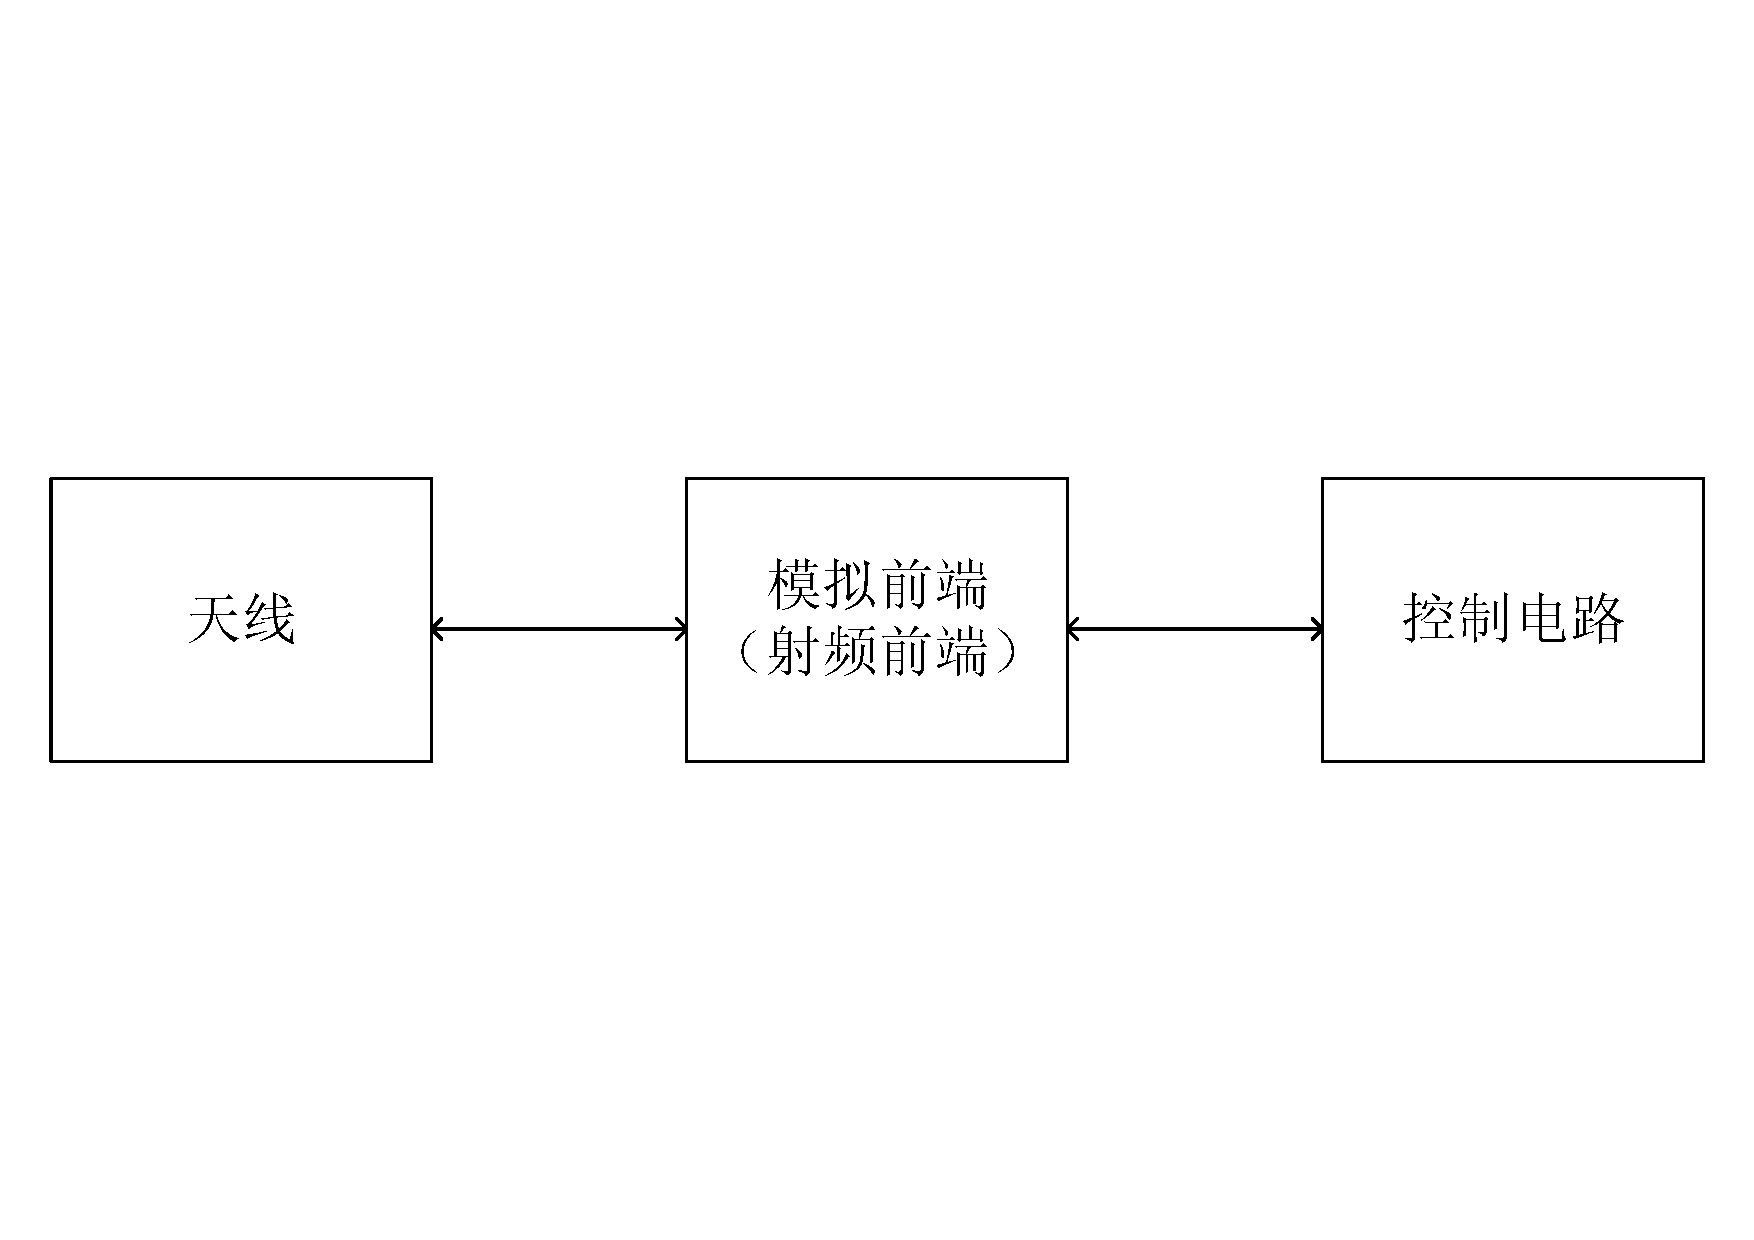
\includegraphics[width=\textwidth, keepaspectratio]{figure/RFID2-0.pdf}\\
	\caption{电子标签的硬件结构(按功能划分)}\label{f0}
\end{figure}

\subsection{读写器的硬件结构简介}
读写器的硬件结构包括射频电路模块和基带电路模块。射频电路模块除了产生高频信号激活电子标签,给电子标签提供能量外,还包括两个独立的收发通道,其中发射通道将按照协议编好的基带信号进行调制并通过天线发送给电子标签,接收通道接收和解调电子标签反馈的微弱的反向散射高频信号并将高频信号还原成基带信号。基带电路由微处理器专用集成电路(Application Specific Integrated Circuit,ASIC)模块构成。ASIC模块专门处理信号的调制和解调等任务。基带电路实现与应用软件通信,完成信号采集处理、运算、编码、解码和校验,执行反碰撞协议算法,对读写器与电子标签之间收发数据进行认证、加密和解密等。应用软件与基带电路之间数据交换可通过USB、RS232、485和以太网等接口,基带电路输出到射频接口的信号是二进制数字信号,而经过射频电路的调制,输出到天线的信号一般是二进制数字信号经过ASK或PSK调制的模拟信号。

\section{高频RFID射频识别标签芯片分析——复旦微电子FM13HS02}
\subsection{芯片简介}
FM13HS02是复旦微电子公司开发的符合ISO/IEC15693协议的ITAG系列高频安全电子标签芯片之一,具较好的射频性能和射频兼容性,保证了更远的操作距离和更可靠的读写。FM13HS02芯片提供了较大容量数据存储空间,内置国家商用密码算法SM7,支持安全鉴别和安全通信。FM13HS02芯片具有物理不可克隆功能(PUF),并创新性的将PUF与SM7算法相结合,显著提升了算法实现的安全性。FM13HS02芯片具有物理唯一性和高安全性的特点,可广泛应用于高值物资管理、防伪溯源、证件、会议通行证等领域。

\subsection{硬件结构}
FM13HS02芯片由模拟射频电路、数字逻辑电路和存储器三部分组成,属于不可编程电子标签,读写器与芯片间的射频接口符合ISO/IEC 15693-2和ISO/IEC 15693-3,其整体结构框图如图\ref{f1}所示:
\begin{itemize}
	\item 模拟射频接口:模拟射频接口即该标签芯片的射频前端,负责接收天线中传来的读写器信号、提取能量、解调读写器信号以及激活并维持系统时钟脉冲、接收并调制数字信号通过天线完成数据回发。
	\item 数字检测电路:数字检测电路是该芯片的主要功能部件。数字逻辑电路负责执行防冲突算法、完成射频前端输入信号的解码、数据的加密和解密、控制对EEPROM的读写、对回发数据的编码以及控制系统时钟。
	\item 非易失性存储器(EEPROM):提供高可靠的数据存储。
\end{itemize}

\begin{figure}
	\centering
	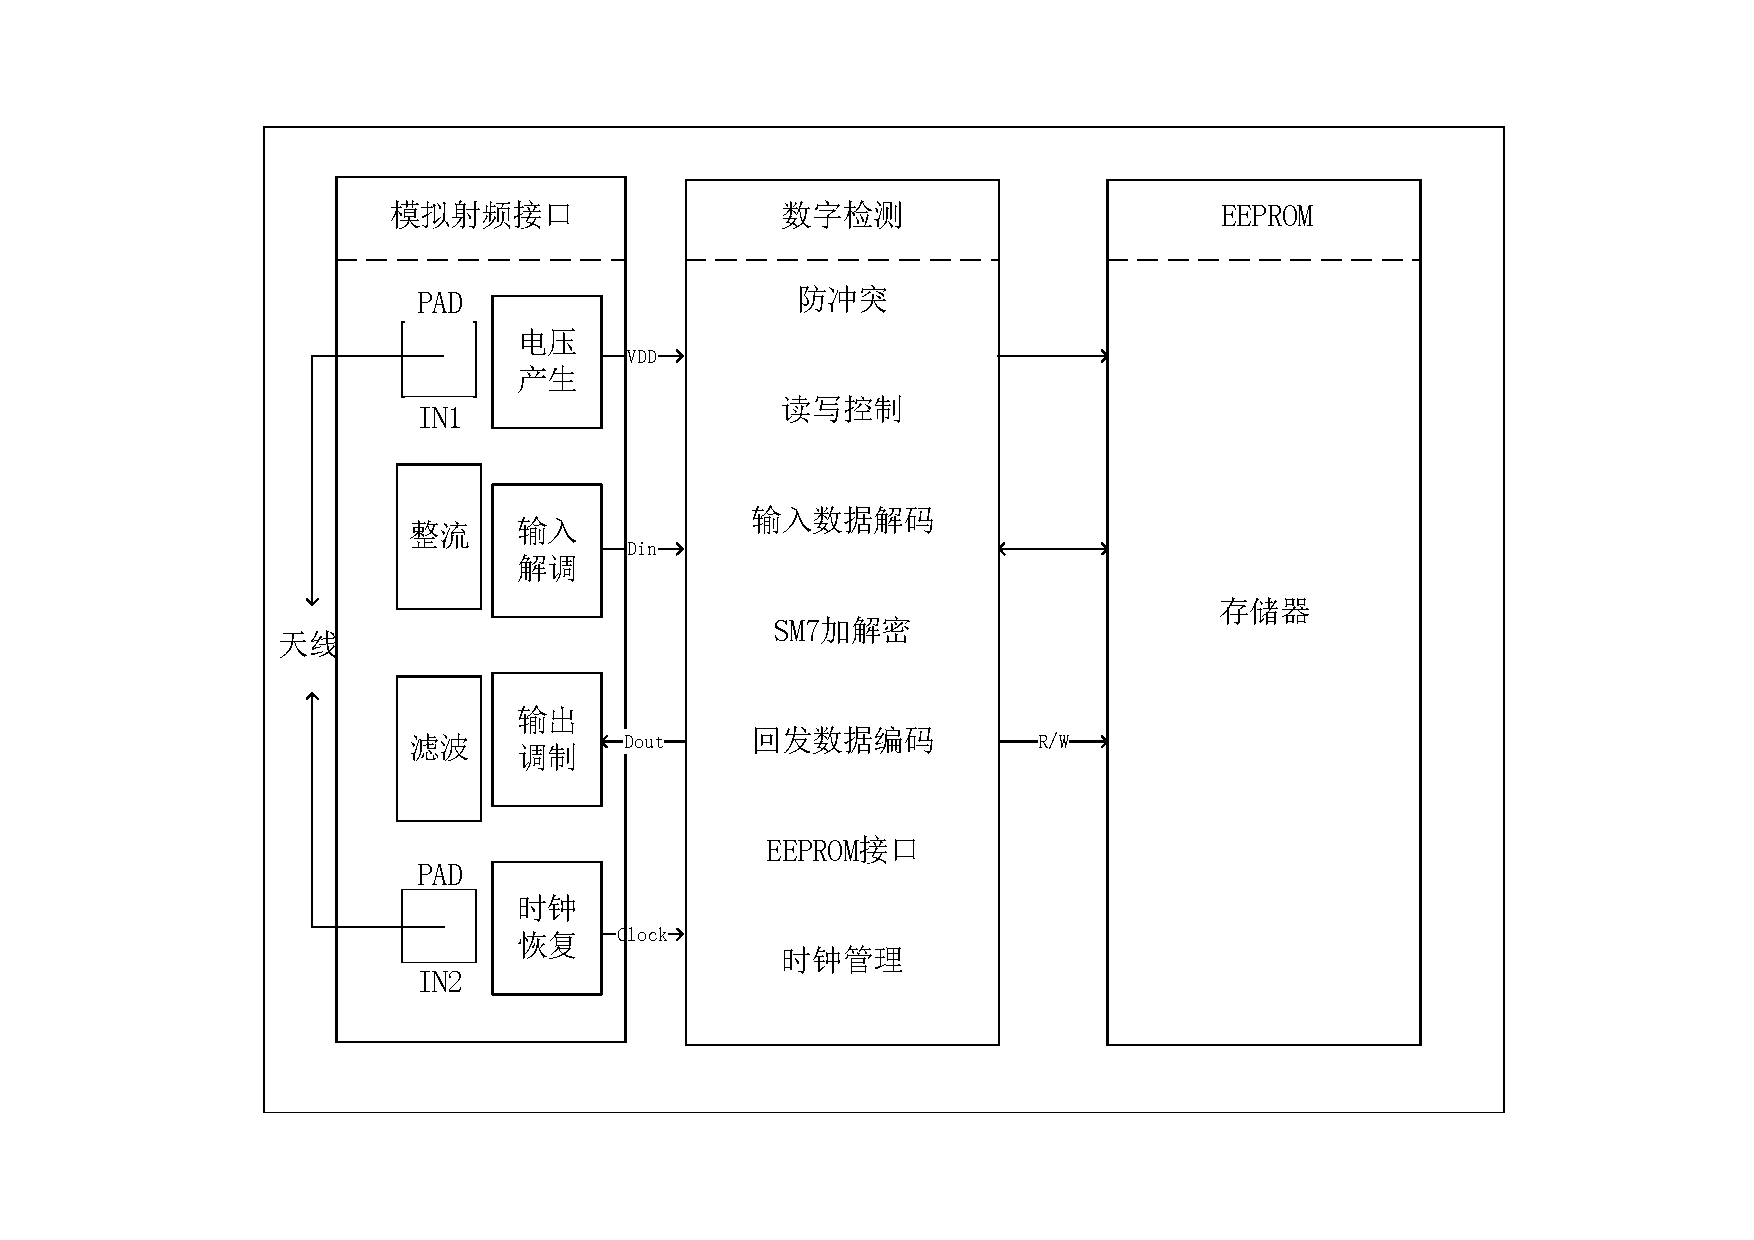
\includegraphics[width=\textwidth, keepaspectratio]{figure/RFID2.pdf}\\
	\caption{复旦微电子FM13HS02芯片结构图}\label{f1}
\end{figure}
\subsection{关键技术分析}
\subsubsection{ISO/IEC 15693标准}
ISO/IEC 15693是一种短距离非接触式IC卡数据协议标准,该标准规定了读取距离可达一米的非接触IC卡的功能及运作模式,使用的频率为13.56MHz,数据传输速率的一般上限是53Kb/s或者26.5Kb/s,采用轮寻机制、分时查询的方式完成防冲突过程。

该标准设计简单,生产读取器的成本比ISO/IEC 14443低,应用场景多为开放式会议签到、考勤等。

\subsubsection{国家商用密码算法}
为了保障商用密码的安全性,国家商用密码管理办公室制定了一系列密码标准\cite{RN100},包括SM1(SCB2)、SM2、SM3、SM4、SM7、SM9、祖冲之密码算法(ZUC)等。其中SM1、SM4、SM7、祖冲之密码(ZUC)是对称算法;SM2、SM9是非对称算法;SM3是哈希算法。目前,这些算法已广泛应用于各个领域中。其中SM1、SM7算法不公开,仅以IP核的形式存在于芯片中,使用该算法时,一般通过加密芯片的接口进行调用。

FM13HS02芯片所使用的SM7算法是一种分组密码算法,分组长度为128比特,密钥长度为128比特\cite{RN101}。SM7适用于非接触式IC卡,应用包括身份识别类应用(门禁卡、工作证、参赛证),票务类应用(大型赛事门票、展会门票),支付与通卡类应用(积分消费卡、校园一卡通、企业一卡通等)。

\subsubsection{物理不可克隆技术}
物理不可克隆技术(Physical Unclonable Function,PUF)利用了芯片制造过程中注入和光照等工序的随机工艺偏差,产生芯片的唯一“指纹”信息,经特殊技术提取后,可作为芯片的唯一标识信息。该唯一标识由于是制造过程中自行产生,芯片的设计者、制造者、生产者均无法对其进行控制,保证了防伪芯片的物理不可复制特性。

芯片为保证自身安全性,需内置加密算法,加密算法除了保证数学上的逻辑安全性以外,还需能抵抗暴力破解攻击、侧信道攻击、重放攻击等各种攻击手段,以避免自身存储的密钥被泄露出去。防护手段的强弱与设计复杂度直接相关,而RFID防伪芯片由于其应用环境的特殊性,难以启用复杂的抗攻击设计来保护其内置的密码算法,导致芯片的安全等级下降\cite{RN103}。而FM13HS02芯片中使用PUF技术提取的“指纹”信息,利用了自然环境中普遍存在的物理扰动,具有较好的随机特性,利用该随机特性,可产生随机PUF KEY\cite{RN105},与SM7密码算法相结合,可显著提升密码算法的抗攻击性能和安全等级\cite{RN102}。

\section{高频RFID射频读写器芯片分析——复旦微电子FM17550}
\subsection{芯片简介}
FM17550是一款高度集成的工作在13.56MHz下的非接触通讯芯片,支持以下3种不同的工作模式。
\begin{itemize}
	\item 支持符合 ISO/IEC 14443 TypeA协议的读写器模式
	\item 支持符合 ISO/IEC 14443 TypeB协议的读写器模式
	\item 支持符合 ISO/IEC 14443A协议的卡片模拟工作模式
\end{itemize}
同时提供了低功耗的外部卡片侦测功能,方便电池供电、需要低功耗工作、并且需要实时处理任意 时刻会进入射频场的外部卡片的读写器设备。 FM17550具有低电压、低功耗、驱动能力强、多接口支持、多协议支持等特点。适用于低功耗、低电压、低成本要求的非接触读写器应用。

\subsection{硬件结构}
FM17550芯片由主机接口控制器、控制寄存器组、FIFO缓冲器和芯片主控制器组成,其结构整体框图如图\ref{f2}所示,各部分功能如下:
\begin{itemize}
	\item 主机接口控制器(Host Interface Control):用于控制芯片与主机的数据交换支持SPI、UART、I2C三种连接方式,所有的接口在上电硬复位之后自动完成接口方式的侦测。
	\item 控制寄存器组(Control Register Bank):包含用于控制芯片各种功能的寄存器单元。
	\item 8*64位FIFO缓冲器(FIFO,codec,Receiver,Transmitter):用于主控芯片与内部状态机之间的输入输出数据流的缓冲。图中的codec,Receiver,Transmitter三者负责缓冲器与该缓冲器与内部状态机之间的数据交换。该缓冲器对于最长64字节的数据流控制非常方便,使数据传输时无需考虑交互时序。
	\item 芯片主控制器(Control Engine):芯片主控制器是FM17550芯片的核心部件,负责控制和协调芯片的大部分处理过程。主控制器又可以分成下列功能单元:
	\begin{itemize}
		\item 加密单元(Encryption Unit):加密单元在读写器模式下负责数据的M1加密;
		\item CRC协处理器(CRC Co-prosesscer):用于对数据进行CRC校验;
		\item 中断控制器(Interrupt Control):处理系统中断信号,控制芯片的中断;
		\item 时钟和reset控制器(Clock/reset control):用于维持稳定的系统时钟以及控制芯片重启;
		\item 可编程定时器(Programable timer):内置的Timer计时单元,主控芯片可以利用该计时器进行计时相关的任务,支持超时计数器、看门狗计数器、秒表、可编程脉冲输出、周期性脉冲触发功能;
		\item 电源控制器(Power Manage Unit):用于控制芯片各组件的电源供应,除支持正常功耗模式外还支持三种低功耗模式,Deep power down模式(DPD)、Hard power down模式(HPD)和Soft power down模式(SPD)。其中,SPD模式下,芯片内部逻辑进入低功耗状态,关闭晶振;HPD模式关闭大部分数字逻辑的供电、关闭晶振,并使所有双向IO引脚都 控制为三态输出,输入引脚隔离与内部电路的连接;DPD模式在HPD模式的基础上进一步关闭所有数字逻辑的供电,使系统能耗尽可能降到最低。
	\end{itemize}
\end{itemize}
\begin{figure}
	\centering
	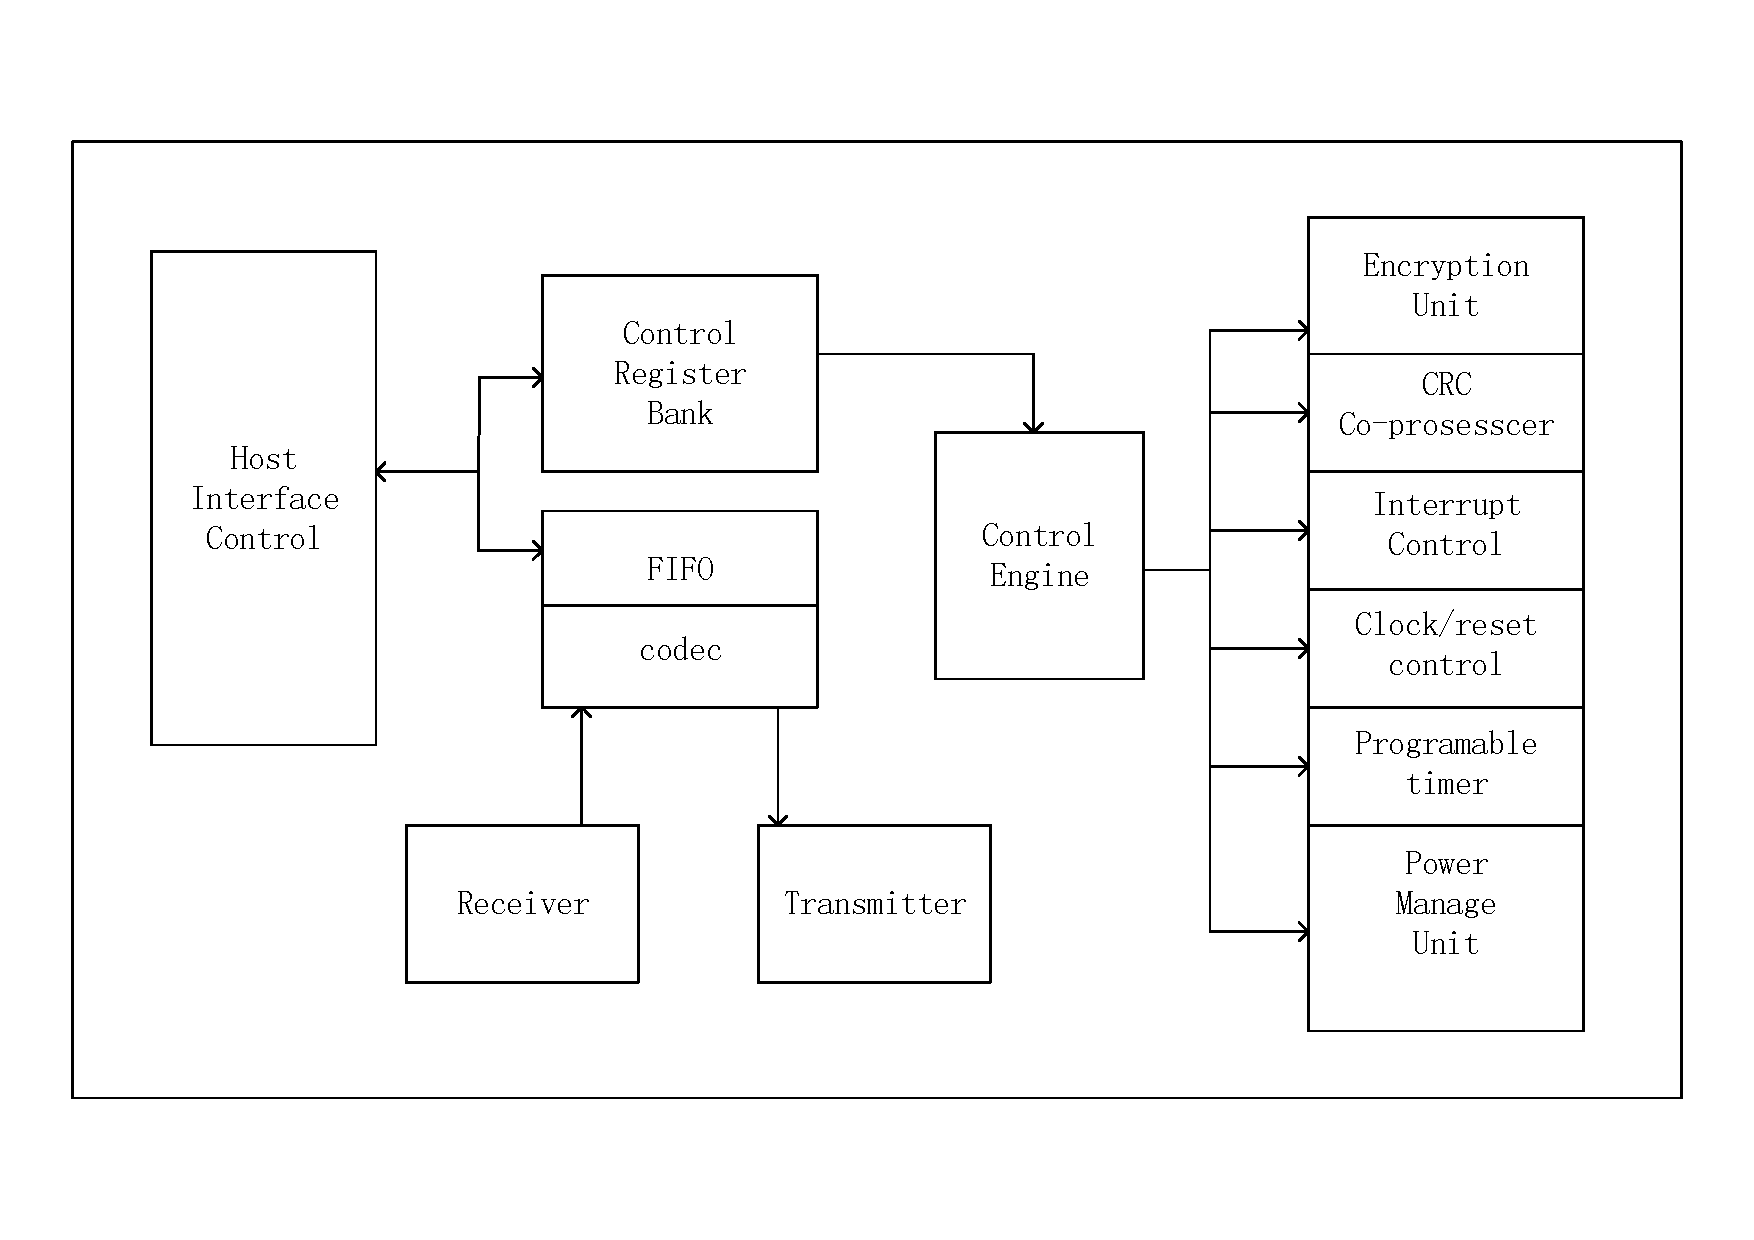
\includegraphics[width=\textwidth]{figure/RFID2-2.pdf}\\
	\caption{复旦微电子FM17550芯片结构图}\label{f2}
\end{figure}

FM17550芯片的QFN32封装方式及引脚定义见附录图\ref{f3}和表\ref{tab:引脚定义}。
\subsection{关键技术分析}
\subsubsection{ISO/IEC14443标准}
ISO/IEC 14443标准是一种超短距离非接触式IC卡标准,规定了读取距离7-15厘米的非接触式IC卡的功能及运作方式,使用的频率为13.56MHz,通信速率为106kbit/s。

ISO/IEC 14443定义了Type A,和Type B两种类型协议,它们的不同主要在于载波的调制深度及位的编码方式:Type A采用开关键控(On-Off keying)的Manchester编码,Type B采用NRZ-L的BPSK编码。Type B与Type A相比,具有传输能量不中断、速率更高、抗干扰能力强的优点。Type A和Type B的防冲突机制原理也有所不同:Type A的防冲突算法基于位冲突检测协议,而Type B使用通信系列命令序列完成防冲突过程。

与ISO/IEC 15693相比,ISO/IEC 14443 读写距离较近,灵敏度较低,但具有加密功能。ISO/IEC 14443 Type A协议的应用领域主要有门禁卡、考勤卡、公交卡、一卡通等,而Type B协议的加密功能更加完善,主要用于身份证、护照、银联卡等需要高安全性和大容量的场合,目前的第二代电子身份证采用的标准就是ISO/IEC 14443 Type B协议。

\addcontentsline{toc}{section}{参考文献}
\bibliography{ref}
\bibliographystyle{unsrt}
\newpage
\addcontentsline{toc}{section}{附录}
\begin{appendices}
\section*{附录}
\subsection*{复旦微电子FM17550芯片封装图和引脚定义}

\begin{figure}[htp]
	\centering
	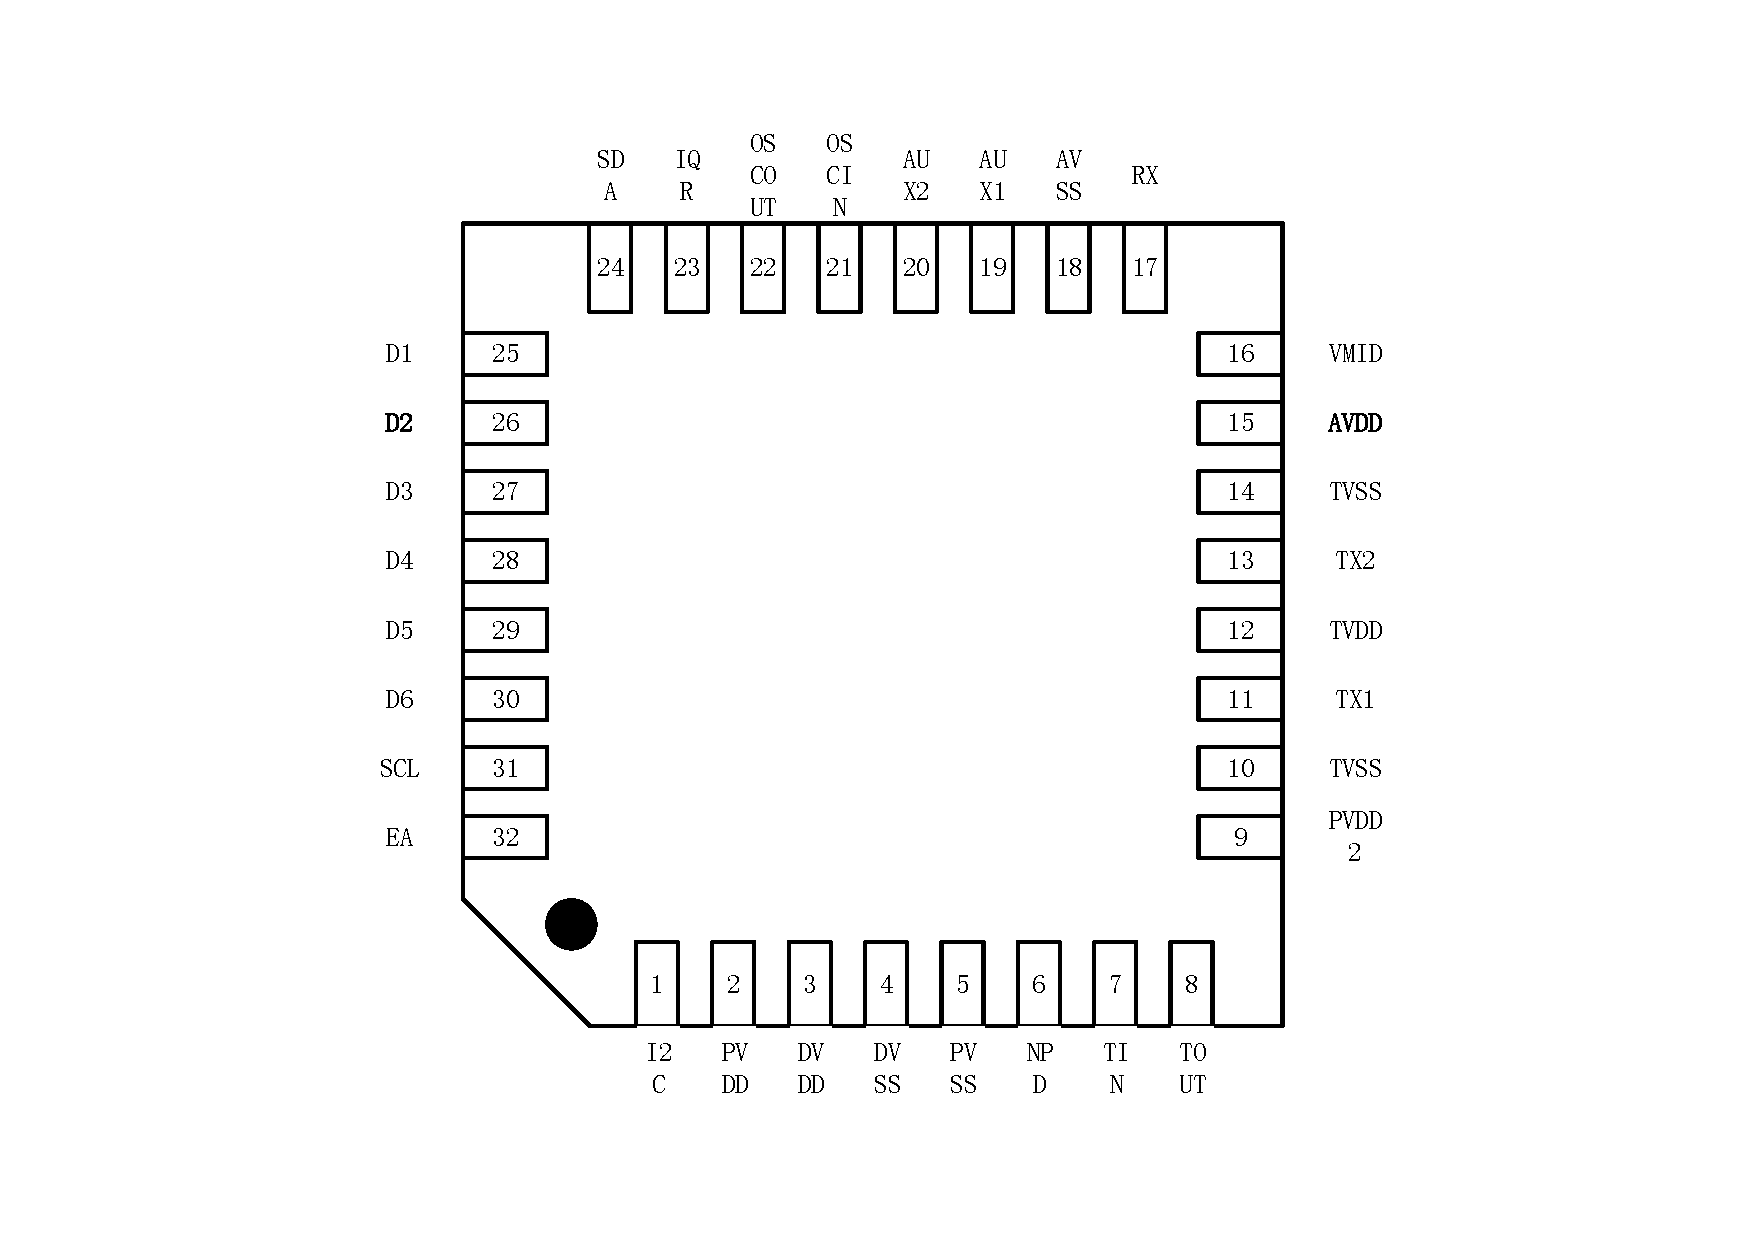
\includegraphics[width=\textwidth]{figure/RFID2-3.pdf}\\
	\caption{复旦微电子FM17550芯片封装图}\label{f3}
\end{figure}

\newpage

\begin{table}[htbp]
	\centering
	\caption{复旦微电子FM17550芯片引脚定义}
	\label{tab:引脚定义}
	\setstretch{1.065}
	\begin{tabular}{|c|c|c|l|}
		\hline
		引脚序号  & 引脚名称  & 类型    & 引脚说明 \\
		\hline
		1     & I2C   & I     & I2C总线接口使能 \\
		\hline
		2     & PVDD  & P     & 引脚供电 \\
		\hline
		3     & DVDD  & P     & 芯片供电 \\
		\hline
		4     & DVSS  & G     & 数字地 \\
		\hline
		5     & PVSS  & G     & 引脚地 \\
		\hline
		      &       &       & \multicolumn{1}{p{23.585em}|}{复位/休眠(Power Down)控制脚} \\
		6     &NPD    & I     & \multicolumn{1}{p{23.585em}|}{电平时内部电路进入power down状态} \\
		      &       &       & \multicolumn{1}{p{23.585em}|}{当产生一个上升沿时内部电路复位} \\
		\hline
		7     & TIN   & I     & 测试信号输入 \\
		\hline
		8     & TOUT  & O     & 测试信号输出 \\
		\hline
		9     & PVDD2 & P     & TIN、TOUT引脚供电 \\
		\hline
		10    & TVSS  & G     & 发射电路地 \\
		\hline
		11    & TX1   & O     & 发射输出脚1 \\
		\hline
		12    & TVDD  & P     & 发射电路供电 \\
		\hline
		13    & TX2   & O     & 发射输出脚2 \\
		\hline
		14    & TVSS  & G     & 发射电路地 \\
		\hline
		15    & AVDD  & P     & 模拟电路供电 \\
		\hline
		16    & VMID  & P     & 为部参考电压 \\
		\hline
		17    & RX    & I     & 射频输入引脚 \\
		\hline
		18    & AVSS  & G     & 模拟地 \\
		\hline
		19    & AUX1  & O     & 测试输出1 \\
		\hline
		20    & AUX2  & O     & 测试输出2 \\
		\hline
		21    & OSCIN & I     & 27.12M晶振输入,也作外部时钟输入 \\
		\hline
		22    & OSCOUT & O     & 27.12M晶振输出 \\
		\hline
		23    & IRQ   & O     & 中断输出 \\
		\hline
		\multirow{3}{*}{24}    & SDA   & IO    & I2C总线数据IO脚 \\
		\cline{2-4}
		& NSS   & I     & SPI接口使能 \\
		\cline{2-4}
		& URX   & I     & UART接口数据输入 \\
		\hline
		\multirow{2}{*}{25}& D1    & IO    & 测试口 \\
		\cline{2-4}
		          & ADR5  & I     & 12C总线地址bit5 \\
		\hline
		\multirow{2}{*}{26}    & D2    & IO    & 测试口 \\
		\cline{2-4}
		          & ADR4  & I     & 12C总线地址bit4 \\
		\hline
		\multirow{2}{*}{27}& D3    & IO    & 测试口 \\
		\cline{2-4}
		          & ADR3  & I     & 12C总线地址bit3 \\
		\hline
		\multirow{2}{*}{28}& D4    & IO    & 测试口 \\
		\cline{2-4}
		          & ADR2  & I     & 12C总线地址bit2 \\
		\hline
		\multirow{4}{*}{29}& D5    & IO    & 测试口 \\
		\cline{2-4}
		          & ADR1  & I     & 12C总线地址bit1 \\
		\cline{2-4}
		          & SCK   & I     & SPI接口时钟输入 \\
		\cline{2-4}
		          & DTRQ  & O     & UART请求输出给mcu \\
		\hline
		\multirow{4}{*}{30}& D6    & IO    & 测试口 \\
		\cline{2-4}
		          & ADRO  & I     & 12C总线地址bit0 \\
		\cline{2-4}
		          & MOSI  & I     & SPI接口master输出slave输入 \\
		\cline{2-4}
		          & MX    & O     & UART输出到mcu \\
		\hline
		\multirow{3}{*}{31}& SCL   & I     & 12C总线时钟线 \\
		\cline{2-4}
		          & MISO  & O     & SPI接口master输入slave输出 \\
		\cline{2-4}
		          & UTX   & O     & UART接口数据输出 \\
		\hline
		32    & EA    & I     & 2C总线地址模式 \\
		\hline
	\end{tabular}
\end{table}
\end{appendices}
\end{spacing}
\end{document}